\documentclass[../main.tex]{subfiles}

\begin{document}

\subsection{Seguridad estructural}
´
Para poder determinar la seguridad de una estructura, podemos hacer un
\textbf{análisis global plástico} y un \textbf{análisis global elástico}.Hasta ahora, 
lo único que hemos visto es el último. Esto implica que nuestras hipótesis 
consideran que las deformaciones y esfuerzos se encuentran dentro del límite elástico.
Esto nos permite hacer cálculos de primer oden y de segundo orden mediante los
efectos de $P-\Delta$ y $P-\delta$).

\subsection{Tipos de estructuras}

Podemos encontrar dos tipos de estrucutras básicas:

\begin{itemize}
  \item \textbf{Estructuras tipo TR:} son aquellas totalmente restringuidas, que
    son diseñadas como pórtico rígido, donde las uniones tienen rigidez 
    suficiente para que los ángulos sean invariables.
  \item \textbf{Estructura tipo TP:} en la cual se supone que las uniones no 
    tienen suficiente rigidez suficiente como para mantener invariables los 
    ángulos entre las barras que concurren.
\end{itemize}

\begin{figure}[ht]
  \centering
  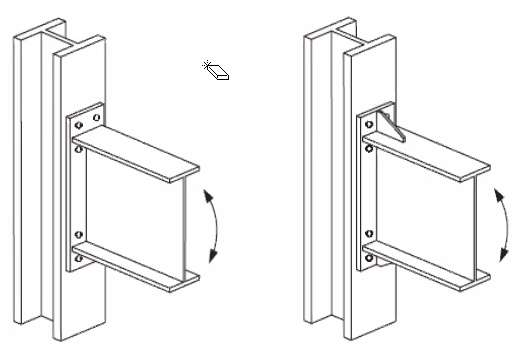
\includegraphics[width=0.8\textwidth]{../images/20210315/esq.png}
  \caption{Esquema de tipos de unión.}
  \label{fig:esq-png}
\end{figure}

\subsection{Coeficiente de seguridad}

El método normalizado para el cálculo del coeficiente de seguridad es a partir
de \textbf{factores de carga y recistencia LRFD}. La ecuanción general es:

\begin{align*}
  \Sigma \gamma_i * Q_i \leq \phi*R_n
.\end{align*}

Donde $\gamma_i$ es el factor de carga, $Q_i$ es el efecto de la carga $i$, y 
$\phi$ es el factor de resistencia. 

El \textbf{grado de seguridad} se puede definir según la estructura de forma que
tenga una aceptable probabilidad de permanecer en servicio durante la vida útil
programada. Debe ser apropiado para que la estructura resista durante su
ejecución y uso.

\subsection{Fuerzas del vientoo}

Este tipo de carga queda reglamentado en el CIRSOC 102. En partícular, existen
dos métodos que podemos utilizar dependiendo de las caracteristicas de la 
estructura a analizar. Estos están definidos en capítulo 4 y 5 de dicho reglamento.

La definición de las mismas viene de un estudio estadistico, y determina cargas
probables. En caso del viento, se trabaja con \textit{presion}, que se calcula
sobre superficies.


\end{document}
